\documentclass[12pt,a4paper]{article}

\usepackage[utf8]{inputenc}
\usepackage[ngerman]{babel}
\usepackage[T1]{fontenc}
\usepackage{amsmath}
\usepackage{amsfonts}
\usepackage{amssymb}
\usepackage{graphicx}
\usepackage[left=2cm,right=2cm,top=2cm,bottom=2cm]{geometry}
\usepackage{multicol}
\usepackage{booktabs}
\usepackage[hidelinks]{hyperref}
\usepackage{tikz}
\usepackage{pgfplots}
\usepackage{blindtext}
\usepackage{array}
\usepackage{multirow}
\usepackage{bigdelim}
\usepackage{colortbl}
\usepackage{fancyhdr} 
\usepackage{tabularx}
\usepackage{xcolor}
\usepackage{color}
\usetikzlibrary{decorations.text}
\usetikzlibrary{tikzmark}
\pagestyle{fancy} 
	\fancyhf{} 
	\fancyhead[L]{
\includegraphics[scale=0.05]{Bilder/dhbw.png}} 
	\fancyhead[C]{\slshape Algorithmen und Komplexitaet} 
	\fancyhead[R]{\slshape LaTeX Version}

\usepackage{helvet}
\renewcommand{\familydefault}{\sfdefault}

\author{\slshape Robin Rausch, Florian Maslowski}
\title{Algorithmen und Komplexität}
\date{\slshape \today}
\begin{document}
\maketitle
\tableofcontents
\newpage
\section{Komplexitaet}
Der Begriff Komplexität beschreibt die Frage:
\begin{quote}
	Wie teuer ist ein Algorithmus?
\end{quote}
Genauergesagt wird hierfür ermittelt, wie viele elementare Schritte eine Algorithmus im Durchschnitt und schlimmstenfalls braucht. Diese beiden Werte spiegeln die Komplexität wieder.
\subsection{$\mathcal{O}$-Notation}
Die $\mathcal{O}$-Notation ist eine obere Grenze einer Funktion. $\mathcal{O}(f)$ ist die Menge aller Funktionen, die langfristig nicht wesentlich schneller wachsen als $f$.
\newline
Einige Beispiele sind zum Beispiel:\newline
\begin{itemize}
	\item $n^2 \in \mathcal{O}(n^3)$
	\item $3n^3 + 2n^2 + 17 \in \mathcal{O}(n^3)$
	\item $n \sqrt{n} \in \mathcal{O}(n^2)$
\end{itemize}
\textbf{Rechenregeln für $\mathcal{O}$-Notation:}
\begin{center}
	\begin{tabularx}{\textwidth}{r c r c l}
		Für jede Funktion $f$ & & $f$ & $\in \mathcal{O}(f)$ & \\
		$g \in \mathcal{O}(f)$ & $\Rightarrow $ & $c \cdot g$ & $\in \mathcal{O}(f)$ & Konstanter Faktor\\
		$g \in \mathcal{O}(f) \wedge h \in \mathcal{O}(f)$ & $\Rightarrow $ & $g + h$ & $\in \mathcal{O}(f)$ & Summe\\
		$g \in \mathcal{O}(f) \wedge h \in \mathcal{O}(g)$ & $\Rightarrow $ & $h$ & $\in \mathcal{O}(f)$ & Transivität\\
		$\lim_{n \to \infty} \frac{g(n)}{f(n)} \in \mathbb{R} $ & $\Rightarrow $ & $g$ & $\in \mathcal{O}(f)$ & Grenzwert\\
	\end{tabularx}
\end{center}

\subsubsection{Landau-Symbole}
\begin{tabularx}{\textwidth}{|l|X|c|}
	\hline
	$g  \in  \Omega (f)$ & $g$ wächst mindestens so schnell wie $f$ & $\lim_{x \to \infty} \frac{f(x)}{g(x)} = c \in \mathbb{R}$ \\
	\hline
	$g  \in  \Theta (f)$ & $g$ wächst genau so schnell wie $f$ & $\lim_{x \to \infty} \frac{g(x)}{f(x)} = c \in \mathbb{R}^{>0}$ \\
	\hline
	$g \sim f$ & $g$ wächst genau so schnell wie $f$ & $\lim_{x \to \infty} \frac{g(x)}{f(x)} = 1$ \\
	\hline
\end{tabularx}
\begin{center}
	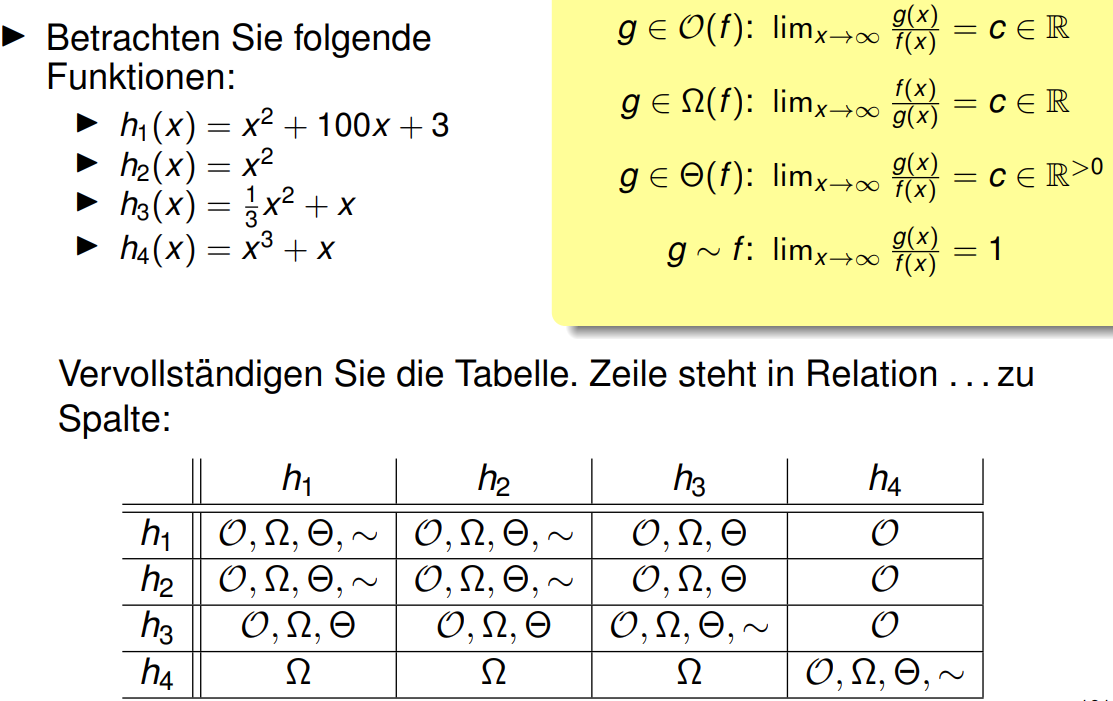
\includegraphics[scale=0.6]{Bilder/landau.PNG}
\end{center}
Zur $\Theta $-Notation gibt es auch ein eigenes \textit{\hyperref[sec:MasterLandau]{Master-Theorem}}.

\subsection{Logarithmen}
Der Logarithmus beschreibt die Umkehrfunktion zur Potenzierung:
\begin{center}
	$\log_a a^b = b$
\end{center}
Wir werden meist den Logarithmus zur Basis 2 brauchen.\newline
Rechenregeln mit dem Logarithmus:
\begin{center}
	$log_ax = \frac{\log_bx}{\log_ba}$\\
	\vspace*{.6cm}
	$\log_ax = \frac{1}{\log_ba}\log_bx = c\log_bx$\\
	\vspace*{.6cm}
	$\mathcal{O}(\log_ax) = \mathcal{O}(c\log_bx) = \mathcal{O}(\log_bx)$ $\Rightarrow $ Die Basis ist für $\mathcal{O}$ irrelevant!
\end{center}

\subsection{Dynamisches Programmieren}
Dynamisches Programmieren ist eine Optimierung der normalen Programmierung. Hierfür werden Probleme in kleinere Teilprobleme aufgeteilt. Die Teilprobleme werden gelöst und dann die Gesamtlösung aus den Teillösungen rekonstruiert.\newline
Die Dynamische Programmierung versagt, wenn...
\vspace{.35cm}
\begin{itemize}
	\item Einzellösungen nicht wiederverwendet werden können
	\item die globale Lösung sich nicht einfach aus lokalen Lösungen zusammensetzen lässt
\end{itemize}
\vspace{.35cm}
Ein Beispiel für die Verwendung der dynamischen Programmierung ist eine rekursive Fibonacci-Funktion.

\subsection{Rekurrenzen}
Rekursion?

\subsection{Divide \& Conquer}
Der Divide \& Conquer-Ansatz teilt ein Problem in zwei gleich große Hälften und muss somit nur noch ein halb so großes Problem lösen.\newline
Ein Algorithmus der...
\begin{itemize}
	\item ein Problem in mehrere Teile aufspaltet
	\item die Teilprobleme (rekursiv) löst
	\item die Teillösungen zu einer Gesamtlösung kombiniert
\end{itemize}

\subsubsection{Komplexität von rekursiven Algorithmen}


\section{Einfache Sortierverfahren}
\subsection*{Selectionsort}
\begin{tabularx}{\textwidth}{l l}
	Speicher: &In-place\\
	Stabilität: &Stabil\\
	Komplexität: &$\mathcal{O}(n^2)$\\
\end{tabularx}
\vspace{.8cm}
\newline
\begin{minipage}[c]{0.7\textwidth}
	\begin{enumerate}
		\item Finde kleinstes Element in Folge($a_0, ...a_{k-1}$)
		\item Vertausche $a_{min}$ mit $a_0$
		\item finde kleinstes Element in Folge($a_1, ...a_{k-1}$)
		\item Vertausche $a_{min}$ mit $a_1$
		\item ...
	\end{enumerate}
\end{minipage}
\begin{minipage}[c]{0.3\textwidth}
	\begin{center}
		\begin{tikzpicture}[scale=0.6]
			\foreach \y in {0,...,4}
			{
				\filldraw[green] (-2.5, 0.5 - \y * 2) rectangle (-2.5 + \y,-0.5 - \y * 2);
				\draw[black,very thick] (-2.5, 0.5 - \y * 2) rectangle (2.5,-0.5 - \y * 2);
				\draw[black,very thick] (-1.5, 0.5 - \y * 2) -- (-1.5,-0.5 - \y * 2);
				\draw[black,very thick] (-0.5, 0.5 - \y * 2) -- (-0.5,-0.5 - \y * 2);
				\draw[black,very thick] (0.5, 0.5 - \y * 2) -- (0.5,-0.5 - \y * 2);
				\draw[black,very thick] (1.5, 0.5 - \y * 2) -- (1.5,-0.5 - \y * 2);
			}
			\node at (-2,0){5};
			\node at (-1,0){8};
			\node at (0,0){3};
			\node at (1,0){9};
			\node at (2,0){1};

			\node at (-2,-2){1};
			\node at (-1,-2){8};
			\node at (0,-2){3};
			\node at (1,-2){9};
			\node at (2,-2){5};
			
			\node at (-2,-4){1};
			\node at (-1,-4){3};
			\node at (0,-4){8};
			\node at (1,-4){9};
			\node at (2,-4){5};
			
			\node at (-2,-6){1};
			\node at (-1,-6){3};
			\node at (0,-6){5};
			\node at (1,-6){9};
			\node at (2,-6){8};
			
			\node at (-2,-8){1};
			\node at (-1,-8){3};
			\node at (0,-8){5};
			\node at (1,-8){8};
			\node at (2,-8){9};

			\draw[red,very thick, <->] (-2,0.5) to[out=60, in=120] (2,0.5);
			\draw[red,very thick, <->] (-1,-1.5) to[out=60, in=120] (0,-1.5);
			\draw[red,very thick, <->] (0,-3.5) to[out=60, in=120] (2,-3.5);
			\draw[red,very thick, <->] (1,-5.5) to[out=60, in=120] (2,-5.5);
		\end{tikzpicture}
	\end{center}
\end{minipage}

\subsection{Insertionsort}

\subsubsection{Indirektes Sortieren}

\subsection{Bubblesort}

\subsection{Quicksort}

\section{Divide \& Conquer Sortierverfahren}

\subsection{Mergesort(Top-Down)}
\begin{tabularx}{\textwidth}{l l}
	Speicher: &Out-of-place\\
	Stabilität: &Stabil\\
	Komplexität: &$\mathcal{O}(n^2)$\\
\end{tabularx}
\vspace{.8cm}
\newline
\begin{minipage}[c]{0.7\textwidth}
	\begin{enumerate}
		\item Wenn |S| $\leq $ 1: gib S zurück
		\item Teile S in zwei gleich lange Folgen L und R
		\item Sortieren L und R(rekursiv)
		\item Vereinige L und R zu S':
		\begin{enumerate}
			\item solange L oder R nicht leer sind:
			\item m:= min($l_1,r_1$)
			\item entferne m aus L bzw. R
			\item hänge m an S' an
		\end{enumerate}
		\item gib S' zurück
	\end{enumerate}
\end{minipage}
\begin{minipage}[c]{0.3\textwidth}
	\begin{center}
		\begin{tikzpicture}[scale=0.6]
			\draw[black,very thick](-2.5,-0.5) rectangle (2.5,0.5);
			\draw[black, very thick](-1.5,-0.5) -- (-1.5,0.5);
			\draw[red, very thick](-0.5,-0.5) -- (-0.5,0.5);
			\draw[black, very thick](0.5,-0.5) -- (0.5,0.5);
			\draw[black, very thick](1.5,-0.5) -- (1.5,0.5);
			\node at (-2,0){5};
			\node at (-1,0){8};
			\node at (0,0){3};
			\node at (1,0){9};
			\node at (2,0){1};

			\draw[black,very thick](-3,-2.5) rectangle (-1,-1.5);
			\draw[black,very thick](0,-2.5) rectangle (3,-1.5);
			\draw[red, very thick](-2,-2.5) -- (-2,-1.5);
			\draw[red, very thick](2,-2.5) -- (2,-1.5);
			\draw[black, very thick](1,-2.5) -- (1,-1.5);
			\node at (-2.5,-2){5};
			\node at (-1.5,-2){8};
			\node at (0.5,-2){3};
			\node at (1.5,-2){9};
			\node at (2.5,-2){1};

			\draw[black,very thick](-3.25,-3.5) rectangle (-2.25,-4.5);
			\draw[black,very thick](-1.75,-3.5) rectangle (-0.75,-4.5);
			\draw[black,very thick](0,-3.5) rectangle (1,-4.5);
			\draw[black,very thick](1.5,-3.5) rectangle (3.5,-4.5);
			\draw[red, very thick](2.5,-3.5) -- (2.5,-4.5);
			\node at (-2.75,-4){5};
			\node at (-1.25,-4){8};
			\node at (0.5,-4){3};
			\node at (2,-4){9};
			\node at (3,-4){1};

			\draw[black,very thick](1.25,-5.5) rectangle (2.25,-6.5);
			\draw[black,very thick](2.75,-5.5) rectangle (3.75,-6.5);
			\node at (1.75,-6){9};
			\node at (3.25,-6){1};

			\draw[green,very thick](1.5,-7.5) rectangle (3.5,-8.5);
			\draw[green,very thick](2.5,-7.5) -- (2.5,-8.5);
			\node at (2,-8){1};
			\node at (3,-8){9};

			\draw[green,very thick](-3,-9.5) rectangle (-1,-10.5);
			\draw[green,very thick](0,-9.5) rectangle (3,-10.5);
			\draw[green, very thick](-2,-9.5) -- (-2,-10.5);
			\draw[green, very thick](2,-9.5) -- (2,-10.5);
			\draw[green, very thick](1,-9.5) -- (1,-10.5);
			\node at (-2.5,-10){5};
			\node at (-1.5,-10){8};
			\node at (0.5,-10){1};
			\node at (1.5,-10){3};
			\node at (2.5,-10){9};

			\draw[green,very thick](-2.5,-11.5) rectangle (2.5,-12.5);
			\draw[green, very thick](-1.5,-11.5) -- (-1.5,-12.5);
			\draw[green, very thick](-0.5,-11.5) -- (-0.5,-12.5);
			\draw[green, very thick](0.5,-11.5) -- (0.5,-12.5);
			\draw[green, very thick](1.5,-11.5) -- (1.5,-12.5);
			\node at (-2,-12){1};
			\node at (-1,-12){3};
			\node at (0,-12){5};
			\node at (1,-12){8};
			\node at (2,-12){9};

			\draw[->,blue,very thick](5,0) -- (5,-12);
		\end{tikzpicture}
	\end{center}
\end{minipage}

\section{Heap Sortierverfahren}

\section{Binäre Suchbäume}

\section{AVL-Bäume}

\section{Hashing und Hashtabellen}

\section{Master-Theorem}

\section{Master-Theorem nach Landau}
\label{sec:MasterLandau}

\end{document}